% !TEX program = xelatex
\documentclass[twocolumn]{article}
\usepackage{ctex}
\usepackage{amsmath}
\usepackage{graphicx}
\usepackage{xcolor}
\usepackage{listings}
\usepackage{geometry}
\usepackage{fancyhdr}
\usepackage{tabularx}
\usepackage{booktabs}
\usepackage{hyperref}

% --- 页面布局 ---
\geometry{a4paper, left=2cm, right=2cm, top=2.5cm, bottom=2.5cm, columnsep=1cm}

% --- 代码高亮配置 ---
\definecolor{codegreen}{rgb}{0,0.6,0}
\definecolor{codegray}{rgb}{0.5,0.5,0.5}
\definecolor{codepurple}{rgb}{0.58,0,0.82}
\definecolor{backcolour}{rgb}{0.95,0.95,0.92}

\lstdefinestyle{mystyle}{
    backgroundcolor=\color{backcolour},   
    commentstyle=\color{codegreen},
    keywordstyle=\color{magenta},
    numberstyle=\tiny\color{codegray},
    stringstyle=\color{codepurple},
    basicstyle=\ttfamily\footnotesize,
    breakatwhitespace=false,         
    breaklines=true,                 
    captionpos=b,                    
    keepspaces=true,                 
    numbers=left,                    
    numbersep=5pt,                  
    showspaces=false,                
    showstringspaces=false,
    showtabs=false,                  
    tabsize=2,
    columns=flexible,
    literate={\_}{{\textunderscore}}1,
    mathescape=false,
    texcl=false
}
\lstset{style=mystyle}

% --- 自定义 listings 语言 ---
\lstdefinelanguage{flex}{
    keywords={%
        options, case-insensitive, noyywrap, yylineno,
        x, s,
    },
    sensitive=false,
    morecomment=[l][\color{codegreen}]{//},
    morecomment=[s][\color{codegreen}]{/*}{*/},
    morecomment=[s][\color{codegreen}]{\%\{}{\%\}},
    morestring=[b][\color{codepurple}]",
    alsoletter={-,>},
    morekeywords=[2]{BEGIN, ECHO, REJECT, yylval, yytext, yyleng, yylex, curr_lineno},
    mathescape=false,
    texcl=false,
}

\lstdefinelanguage{cool}{
    keywords={%
        class, inherits, if, then, else, fi, while, loop, pool, let, in, case, of, esac, new, isvoid, not, true, false,
        Int, String, Bool, Object, SELF_TYPE, self
    },
    sensitive=false,
    morecomment=[l][\color{codegreen}]{--},
    morecomment=[s][\color{codegreen}]{(*}{*)},
    morestring=[b][\color{codepurple}]",
    morekeywords=[2]{},
}


% --- 页眉页脚 ---
\pagestyle{fancy}
\fancyhf{}
\fancyhead[L]{COOL 词法分析器实验报告}
\fancyhead[R]{\thepage}
\fancyfoot[C]{\small \copyright\ 2025}
\renewcommand{\headrulewidth}{0.4pt}
\renewcommand{\footrulewidth}{0.4pt}

% --- 标题 ---
\title{
    \vspace{-1cm} % 调整标题位置
    \textbf{COOL 语言词法分析器开发报告} \\
    \large \texttt{Compiler Principle Assignment}
}
\author{
    姓名: \textcolor{red}{谭润} \\
    学号: \textcolor{red}{20238131027} \\
    班级: \textcolor{red}{大数据二班}
}
\date{\today}

% --- 文档开始 ---
\begin{document}

\maketitle
\thispagestyle{fancy} % 首页也使用fancy样式

\begin{abstract}
\noindent
(自己根据情况改改)
本文档详细记录了 COOL (Classroom Object-Oriented Language) 词法分析器的设计与实现过程。报告首先深入阐述Flex词法分析器的工作原理,包括有限状态自动机理论、模式匹配机制和状态转换过程;然后详细说明词法规则的实现方法,涵盖关键字、标识符、字符串、注释及错误处理;最后通过完整的测试验证,包括集成测试,展示词法分析器与编译器其他组件的协作以及最终程序的正确运行。

\textcolor{red}{%
% TODO: 请根据你的实际工作,简要修改摘要内容。特别注意强调你对Flex原理的理解。
}
\end{abstract}

\section{项目概述与环境}
\subsection{项目目标}
(自己根据情况改改)
本次作业的目标是使用词法分析器生成工具 Flex 为 COOL 语言设计并实现一个完整的词法分析器。该分析器需要能够将 COOL 源代码文本文件转换为一个词法单元(Token)序列,并能正确处理各种边界情况和词法错误。

\subsection{开发环境}

\textcolor{red}{%
% TODO: 请详细填写以下开发环境信息
}

\subsubsection{硬件配置(云服务器信息)}
\begin{itemize}
    \item \textbf{CPU}: \textcolor{red}{x86_64架构,2核}
    \item \textbf{内存}: \textcolor{red}{总容量2.0Gi}
    \item \textbf{硬盘}: \textcolor{red}{根分区容量总计约 11G(文件系统为 ext4)}
\end{itemize}

\subsubsection{软件环境}
\begin{itemize}
    \item \textbf{操作系统}: \textcolor{red}{Ubuntu 22.04.1 LTS}
    \item \textbf{内核版本}: \textcolor{red}{5.15.0-60-generic}
    \item \textbf{Flex 版本}: \textcolor{red}{2.6.4-8build2}
    \item \textbf{G++ 版本}: \textcolor{red}{g++ (Ubuntu 11.3.0-1ubuntu1~22.04) 11.3.0}
    \item \textbf{Make 版本}: \textcolor{red}{GNU Make 4.3}
    \item \textbf{SPIM 版本}: \textcolor{red}{SPIM Version 8.0 of January 8, 2010}
    \item \textbf{coolc 编译器版本}: \textcolor{red}{0.1}
    \item \textbf{vscode 编辑器版本}: \textcolor{red}{vscode 1.105.1(user setup)}
\end{itemize}

\subsubsection{项目目录结构}
\textcolor{red}{%
% TODO: 使用 tree 命令或手动列出你的项目目录结构
}
\begin{verbatim}
/usr/class/assignments/PA2/(根据你情况)
|-- cool.flex       
|-- test.cl           
|-- lexer             
|-- cool-lex.cc       
|-- Makefile           
|-- parser             
|-- semant            
`-- cgen              
\end{verbatim}

\subsubsection{环境配置过程}

\textcolor{red}{
安装各种依赖包:
\begin{verbatim}
sudo dpkg --add-architecture i386 
sudo apt update 
sudo apt install libc6:i386 
sudo apt install lib32z1 
sudo apt install zlib1g:i386 
sudo apt install libncurses5:i386
\end{verbatim}

安装各种工具:
\begin{verbatim}
sudo apt install flex
sudo apt install spim
\end{verbatim}

安装 coolc 编译器:
\begin{verbatim}
git clone https://github.com/aweinert/coolc.git
sudo apt install openjdk-11-jdk
sudo apt install maven
\end{verbatim}

环境变量持久性设置:
\begin{verbatim}
vim ~/.bashrc
\end{verbatim}
}

% 插入环境变量配置截图
\begin{figure}[htbp]
    \centering
    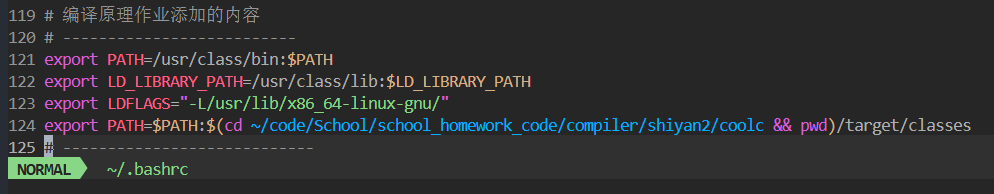
\includegraphics[width=0.9\textwidth]{env.png}
    \caption{环境变量配置内容}
    \label{fig:env_config}
\end{figure}

\textcolor{red}{
环境变量具体配置内容:
\begin{verbatim}
export PATH=/usr/class/bin:$PATH
export LD_LIBRARY_PATH=/usr/class/lib:$LD_LIBRARY_PATH  
export LDFLAGS="-L/usr/lib/x86_64-linux-gnu/"
\end{verbatim}
}

\section{Flex词法分析器原理}

\subsection{Flex工作流程}

\textcolor{red}{%
Flex从.flex文件到可执行词法分析器的完整流程:
\begin{figure}[htbp]
    \centering
    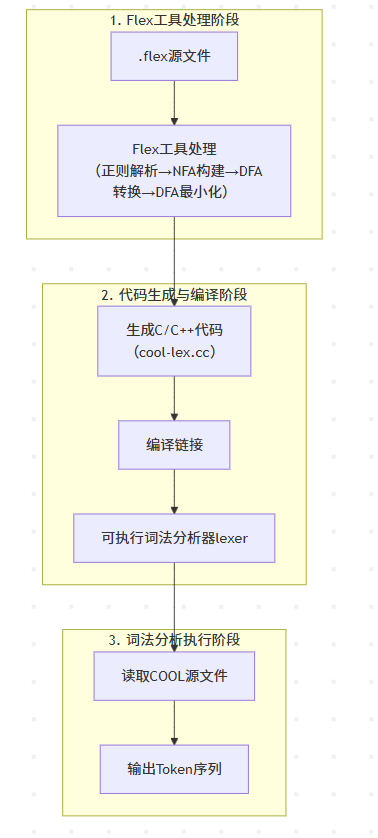
\includegraphics[width=0.8\textwidth]{Flex_work.png}
    \caption{Flex词法分析器工作流程图}
    \label{fig:flex_workflow}
\end{figure}
详细步骤说明:
1.读取.flex文件:Flex读取包含正则表达式规则和动作代码的源文件
2.规则解析:Flex解析三个部分(定义段、规则段、用户代码段)
3.自动机生成:
    a.将正则表达式转换为NFA(非确定有限自动机)
    b.通过子集构造法将NFA转换为DFA(确定有限自动机)
    c.对DFA进行最小化优化
4.代码生成:生成cool-lex.cc文件,包含DFA表和匹配逻辑
5.编译链接:使用g++编译生成可执行文件lexer
6.词法分析:lexer读取COOL源代码,输出Token序列
}

\subsection{有限状态自动机(FSA)原理}

\textcolor{red}{%
% TODO: 详细阐述有限状态自动机的原理:
FSA基本概念: 有限状态自动机是由状态集合、输入字母表、状态转移函数、初始状态和接受状态组成的数学模型
NFA(非确定有限自动机)与 DFA(确定有限自动机)的区别主要体现在:NFA 一个状态对同一输入可有多条转移、允许空串转移、匹配时需回溯效率较低但易于从正则表达式构建;而 DFA 每个状态对每个输入只有唯一转移、不允许空串转移、无回溯匹配效率高且需通过 NFA 转换得到。

\begin{figure}[htbp]
    \centering
    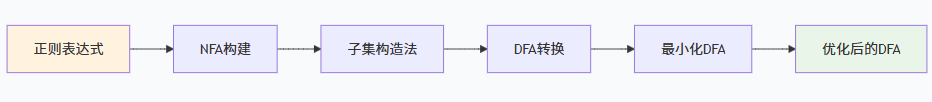
\includegraphics[width=0.8\textwidth]{Flex_auto_create.png}
    \caption{Flex的自动机构建过程}
    \label{fig:flex_workflow}
\end{figure}

示例: 识别整数 "[0-9]+" 的自动机

\begin{figure}[htbp]
    \centering
    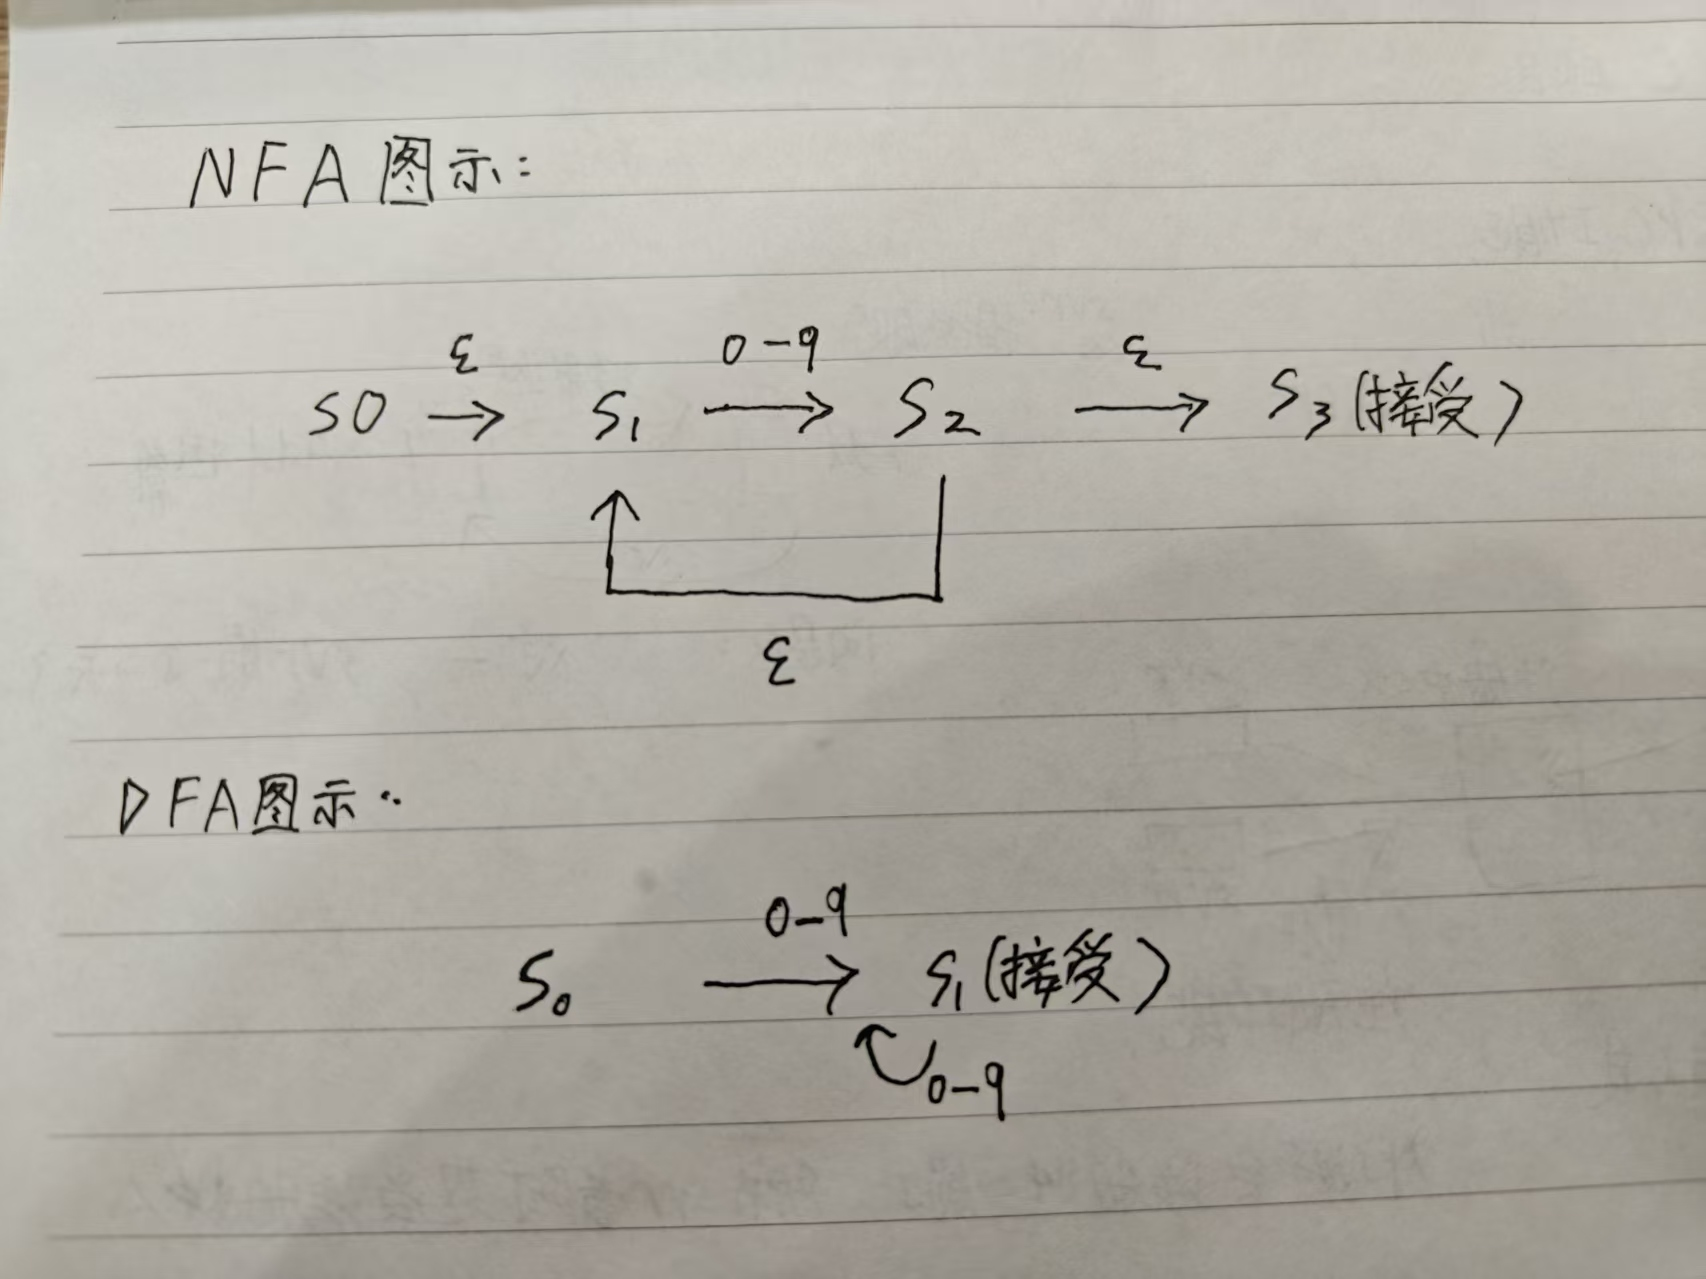
\includegraphics[width=0.8\textwidth]{example1.jpg}
    \caption{识别整数[0-9]+的自动机图示}
    \label{fig:flex_workflow}
\end{figure}
转换过程说明:
1.NFA构建:使用Thompson算法从正则表达式构建NFA
2.子集构造:将NFA状态集合作为DFA的单个状态
3.DFA最小化:合并等价状态,减少状态数量
为什么DFA效率更高:
1.DFA在匹配时不需要回溯,每个输入字符只需一次状态转移
2.NFA可能需要尝试多条路径,存在回溯开销
}

\subsection{模式匹配机制}

Flex使用以下机制进行模式匹配:

\subsubsection{最长匹配原则(Longest Match)}
Flex总是选择匹配最长输入串的规则。

\begin{lstlisting}[language=Flex, caption={最长匹配原则示例}]
%%
"if"     { return IF; }      // 匹配"if"
"ifelse" { return IFELSE; }  // 匹配"ifelse"(更长)
[a-z]+   { return ID; }      // 匹配其他标识符
%%
\end{lstlisting}

\textbf{示例:}输入"ifelse"时,会匹配"ifelse"而不是先匹配"if"。

\subsubsection{规则优先级(First Match)}
当多个规则匹配相同长度时,先定义的规则优先。

\textbf{关键示例:关键字vs标识符}

\begin{lstlisting}[language=Flex, caption={正确的规则顺序}]
// 正确顺序:关键字在前
"if"     { return IF; }      // 优先匹配
"while"  { return WHILE; }   // 优先匹配  
[a-z]+   { return ID; }      // 通用模式在后
\end{lstlisting}

\begin{lstlisting}[language=Flex, caption={错误的规则顺序}]
// 错误顺序:标识符在前
[a-z]+   { return ID; }      // 会匹配所有小写字母串,包括关键字
"if"     { return IF; }      // 永远不会执行!
\end{lstlisting}

\subsubsection{在代码中的体现}
\begin{lstlisting}[language=C++, caption={你代码中的模式匹配实现}]
[cC][lL][aA][sS][sS] { return CLASS; }
// ... 其他关键字
{DAXIEZIMU}{ZIMUSHIZI}* { 
    kulouyylval.symbol = strdup(yytext);
    return TYPEID;
}
{XIAOXIEZIMU}{ZIMUSHIZI}* { 
    kulouyylval.symbol = strdup(yytext);
    return OBJECTID;
}
\end{lstlisting}

\subsubsection{核心变量作用}
\begin{itemize}
    \item \textbf{\texttt{yytext}}:指向当前匹配的文本字符串
    \item \textbf{\texttt{yyleng}}:匹配文本的长度
    \item \textbf{\texttt{yylval}}:用于向语法分析器传递Token值(在你的代码中是\texttt{kulouyylval})
\end{itemize}


\subsection{状态与状态转换}

Flex的状态机制允许词法分析器在不同的上下文中使用不同的匹配规则,这对于处理复杂的词法结构至关重要。

\subsubsection{Flex状态类型}
\begin{itemize}
    \item \textbf{INITIAL}:默认初始状态
    \item \textbf{独占状态(\%x)}:只有明确标记为该状态的规则才会被匹配
    \item \textbf{包容状态(\%s)}:该状态的规则 + 无状态标记的规则都会匹配
\end{itemize}

\subsubsection{状态声明(你的代码)}
\begin{lstlisting}[language=Flex, caption={状态声明}]
%x ZIFUCHUAN    // 独占状态:处理字符串
%x ZHUSHI       // 独占状态:处理注释
\end{lstlisting}

\subsubsection{状态转换机制}
\texttt{BEGIN(state)}宏用于切换状态,改变Flex的匹配规则集合。

\subsubsection{字符串处理状态转换图}
\begin{figure}[H]
    \centering
    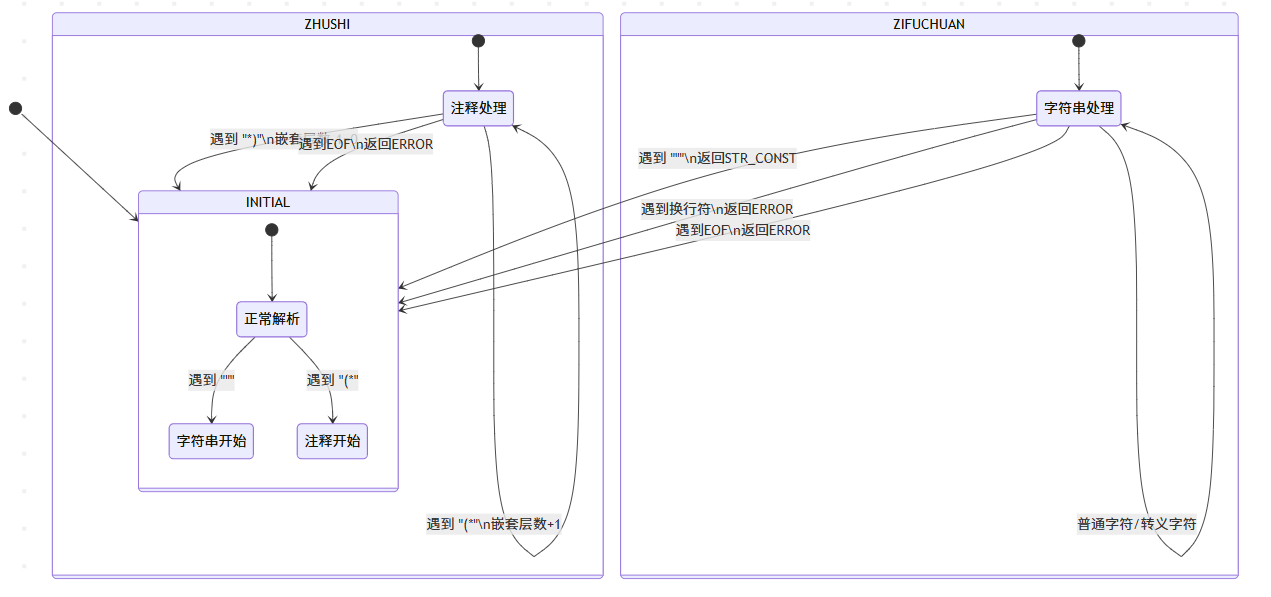
\includegraphics[width=0.9\textwidth]{status_change.png}
    \caption{字符串处理状态转换图}
    \label{fig:status_change}
\end{figure}

\subsubsection{状态转换具体过程(以STRING状态为例)}

\textbf{从INITIAL进入STRING:}
\begin{lstlisting}[language=Flex, caption={进入STRING状态}]
"\"" { 
    BEGIN(ZIFUCHUAN); 
    zifuchuanhuanchongquzhizhen = zifuchuanhuanchongqu; 
}
\end{lstlisting}

\textbf{在STRING状态中处理不同字符:}
\begin{lstlisting}[language=Flex, caption={STRING状态中的字符处理}]
<ZIFUCHUAN>"\"" { 
    *zifuchuanhuanchongquzhizhen = '\0';
    kulouyylval.symbol = strdup(zifuchuanhuanchongqu);
    BEGIN(INITIAL);
    return STR_CONST;
}
<ZIFUCHUAN>\\n { *zifuchuanhuanchongquzhizhen++ = '\n'; }  // 转义处理
<ZIFUCHUAN>\n { 
    dangqianhanghao++; 
    kulouyylval.error_msg = "Unterminated string constant";
    BEGIN(INITIAL);
    return ERROR;
}
\end{lstlisting}

\textbf{返回INITIAL状态:}
\begin{itemize}
    \item 遇到结束引号:\texttt{BEGIN(INITIAL)}并返回\texttt{STR\_CONST}
    \item 遇到错误情况(换行、EOF):\texttt{BEGIN(INITIAL)}并返回\texttt{ERROR}
\end{itemize}

\subsubsection{为什么需要状态机制}
\begin{itemize}
    \item \textbf{上下文相关处理}:字符串内的空格和注释内的关键字不应被正常解析
    \item \textbf{嵌套结构}:注释可以嵌套\texttt{(* outer (* inner *) outer *)}
    \item \textbf{复杂词法结构}:字符串转义、多行注释等需要特殊处理
\end{itemize}


\section{实现细节}
本节简要说明词法规则的实现思路。完整代码见附录。

\subsection{关键字与标识符}

\textbf{基本要求:}
\begin{itemize}
    \item 关键字(如class、if、while等)是大小写不敏感的
    \item 布尔常量true和false的首字母必须小写
    \item TYPE\_ID以大写字母开头,OBJECT\_ID以小写字母开头
    \item 整数常量为数字序列
\end{itemize}

\textcolor{red}{%
% TODO: 说明你如何实现关键字的大小写不敏感、如何区分两种标识符。
% 特别说明:如何处理关键字与标识符的优先级问题。
}


\subsection{字符串处理}

\textbf{基本要求:}
\begin{itemize}
    \item 字符串以双引号开始和结束,不能跨行
    \item 支持转义字符:\texttt{\textbackslash n}, \texttt{\textbackslash t}, \texttt{\textbackslash b}, \texttt{\textbackslash f}, \texttt{\textbackslash"}, \texttt{\textbackslash\textbackslash}
    \item 最大长度1024字符,不能包含空字符
    \item 需要使用Flex状态机(\texttt{\%x STRING})处理
\end{itemize}

\textcolor{red}{%
% TODO: 详细说明你的字符串状态机设计:
% 1. 如何进入和退出STRING状态
% 2. 如何处理各种转义字符
% 3. 如何检测和报告错误(未闭合、过长、包含空字符、EOF等)
% 4. 如何使用字符串缓冲区
}

\subsection{操作符与注释}

\textbf{基本要求:}
\begin{itemize}
    \item 多字符操作符:\texttt{<-}、\texttt{<=}、\texttt{=>}
    \item 单行注释:\texttt{--}到行尾
    \item 多行注释:\texttt{(* *)},支持嵌套
    \item 忽略空白字符,换行时更新行号
\end{itemize}

\textcolor{red}{%
% TODO: 说明你如何处理:
% 1. 多字符操作符与单字符操作符的优先级
% 2. 嵌套注释的实现(使用计数器跟踪嵌套层数)
% 3. 行号的正确更新
}

\subsection{错误处理}

\textbf{需要检测的错误:}
\begin{itemize}
    \item 未闭合的字符串、字符串过长、字符串中的空字符
    \item EOF在字符串或注释中
    \item 未匹配的注释结束符\texttt{*)}
    \item 源代码中的非法字符
\end{itemize}

\textcolor{red}{%
% TODO: 说明你如何检测和报告各种错误,如何设置error\_msg,如何从错误中恢复。
}

\section{测试与验证}
为了验证词法分析器的正确性,我设计了多个测试用例,并使用了项目提供的测试工具。

\subsection{基础功能测试}

测试目标:验证关键字、标识符、常量、操作符的正确识别。

\textcolor{red}{%
% TODO: 编写测试文件test.cl,运行 ./lexer test.cl 或 make dotest,将输出贴在下方。
}

\textbf{测试用例}(test\_basic.cl):
\begin{lstlisting}[language=cool, caption={基础功能测试}]
class Main {
    x : Int <- 42;
    flag : Bool <- true;
    main() : Int { x };
};
\end{lstlisting}

\textbf{测试命令:}
\begin{verbatim}
$ ./lexer test_basic.cl
\end{verbatim}

\textbf{实际输出结果:}
\textcolor{red}{%
% TODO: 将实际的lexer输出贴在这里,应该类似:
}
\begin{verbatim}
#name "test_basic.cl"
#1 CLASS
#1 TYPEID Main
#1 '{'
#2 OBJECTID x
#2 ':'
#2 TYPEID Int
#2 ASSIGN
#2 INT_CONST 42
#2 ';'
#3 OBJECTID flag
#3 ':'
#3 TYPEID Bool
#3 ASSIGN
#3 BOOL_CONST true
#3 ';'
#4 OBJECTID main
...
\end{verbatim}

\subsection{字符串与注释测试}

测试目标:验证字符串转义字符、嵌套注释、各种错误检测。

\textcolor{red}{%
% TODO: 编写包含字符串和注释的测试文件,运行词法分析器,将输出贴在下方。
}

\textbf{测试用例}(test\_string.cl):
\begin{lstlisting}[language=cool, caption={字符串测试}]
(* 测试注释 (* 嵌套注释 *) *)
class Test {
    str1 : String <- "Hello\nWorld";  -- 转义字符
    str2 : String <- "Quote\"Test\"";
};
\end{lstlisting}

\textbf{测试命令与输出:}
\begin{verbatim}
$ ./lexer test_string.cl
\end{verbatim}

\textcolor{red}{%
% TODO: 贴上实际输出,验证:
% 1. 注释被正确忽略
% 2. 字符串正确识别,转义字符处理正确
% 3. STR_CONST token包含转义后的内容
}
\begin{verbatim}
#name "test_string.cl"
#2 CLASS
#2 TYPEID Test
#2 '{'
#3 OBJECTID str1
#3 ':'
#3 TYPEID String
#3 ASSIGN
#3 STR_CONST "Hello\nWorld"
...
\end{verbatim}

\subsection{错误处理测试}

测试目标:验证各种错误情况的检测和报告。

\textcolor{red}{%
% TODO: 测试各种错误情况,每个错误单独测试,展示错误输出。
}

\textbf{测试1:未闭合字符串}
\begin{verbatim}
测试代码:class Main { str : String <- "unclosed
输出:#1 ERROR "Unterminated string constant"
\end{verbatim}

\textbf{测试2:未匹配的注释结束符}
\begin{verbatim}
测试代码:class Main { x : Int; *) }
输出:#1 ERROR "Unmatched *)"
\end{verbatim}

\textbf{测试3:EOF在注释中}
\begin{verbatim}
测试代码:(* comment without closing
输出:#1 ERROR "EOF in comment"
\end{verbatim}

%TODO:  其他内容

\subsection{集成测试}

\textbf{本部分占15分,是评分重点!}

测试目标:验证词法分析器能与编译器其他阶段(语法分析、语义分析、代码生成)正确协作,最终生成可运行的MIPS汇编代码。

\textcolor{red}{%
% TODO: 编写多个完整的COOL程序,展示完整的编译和运行过程:
% 1. 至少包含2-3个不同复杂度的测试程序
% 2. 展示完整的编译命令和输出
% 3. 展示SPIM运行结果
% 4. 说明词法分析器在整个编译流程中的作用
% 5. 如果遇到问题,说明如何调试和解决
}

\textbf{测试程序}(hello.cl):
\begin{lstlisting}[language=cool, caption={集成测试程序}]
class Main inherits IO {
    main() : Object {
        out_string("Hello, COOL!\n")
    };
};
\end{lstlisting}

\textbf{编译过程:}
\begin{verbatim}
$ ./mycoolc hello.cl
\end{verbatim}

\textcolor{red}{%
% TODO: 如果编译成功,应该生成hello.s文件。贴出编译信息(如果有)。
% 如果有警告或错误,说明问题并解决方案。
}

\textbf{运行结果:}
\begin{verbatim}
$ spim hello.s
SPIM Version 8.0 of January 8, 2010
Copyright 1990-2010, James R. Larus.
All Rights Reserved.
Loaded: /usr/class/lib/trap.handler
Hello, COOL!
COOL program successfully executed
\end{verbatim}

\textbf{测试结论:}
\textcolor{red}{%
% TODO: 总结集成测试结果,说明词法分析器与编译器其他部分配合正常。
}

词法分析器成功识别了所有Token,编译器顺利完成了语法分析、语义分析和代码生成,生成的MIPS汇编代码在SPIM模拟器上正确执行,输出了预期结果。这证明词法分析器的实现是正确和完整的。

\section{遇到的问题与解决方案}
\textcolor{red}{%
% TODO: (可选,但建议填写)描述你在开发过程中遇到的主要挑战。
% 例如:
% 1. 对Flex状态机理解不深导致的问题。
% 2. 规则优先级问题(关键字 vs 标识符)。
% 3. C++与Flex的集成问题。
% 简单说明你是如何解决这些问题的。这能很好地体现你的学习和解决问题的能力。
}

\section{总结}
通过本次实验,我深入理解了词法分析的理论基础和Flex工具的工作原理。从有限状态自动机的理论出发,理解了Flex如何将正则表达式转换为高效的DFA,如何进行模式匹配和状态转换。在实践中,我成功实现了一个功能完整且健壮的COOL语言词法分析器,特别是掌握了状态管理机制在处理复杂词法结构时的应用。通过完整的集成测试,我验证了词法分析器能够与编译器其他组件正确协作,最终生成可执行的MIPS代码。这次实验让我对编译器前端有了全面而深刻的认识。

\textcolor{red}{%
% TODO: 根据你的真实感受修改总结。重点总结:
% 1. 对Flex原理的理解和收获
% 2. 对有限状态自动机理论的认识
% 3. 实现过程中的主要挑战和解决方法
% 4. 对整个编译流程的理解
}

\appendix
\section{附录: cool.flex 完整源码}
\label{sec:appendix_code}

\textcolor{red}{%
% TODO: 将你完成的cool.flex文件放在与此tex文件相同的目录下。
% 重新编译后,完整代码会自动包含在这里。
}

\IfFileExists{cool.flex}
  {\lstinputlisting[language=flex, basicstyle=\ttfamily\tiny]{cool.flex}}
  {
\textbf{说明:}将完成的 \texttt{cool.flex} 文件放在同一目录下,重新编译即可自动包含完整代码。

示例结构(3段式):定义段 -- 规则段 -- 用户代码段
}

\end{document}
